% =========================================================
% DIAGRAMA: Ciclo completo petición OBD-II (App → BLE → RPi → CAN → ECU)
% Archivo imagen: Ilustraciones/obd2_cycle.png
%
% QUÉ DIBUJAR EN DRAW.IO:
%   Diagrama de secuencia con 4 actores verticales:
%   [App Móvil] ←BLE→ [Raspberry Pi] ←CAN→ [Arduino ECU Sim]
%
%   Flujo para comando "snapshot" (lectura RPM como ejemplo):
%
%   App ──[ JSON: {"cmd":"snapshot"} ]──────────────────► RPi
%       (BLE NUS write-with-response, MTU 240 bytes)
%
%   RPi ──[ CAN: 7E0 02 01 0C AA AA AA AA AA ]──────────► ECU
%       (ISO-TP SF, Mode 01 PID 0x0C = RPM)
%
%   ECU ──[ CAN: 7E8 04 41 0C 1A F0 AA AA AA ]──────────► RPi
%       (ISO-TP SF response, RPM = (0x1AF0)/4 = 1724 rpm)
%
%   RPi  [decodifica: 1724.0 rpm]
%
%   RPi ──[ JSON: {"pid":12,"name":"Engine RPM","value":1724.0,"unit":"rpm"} ]─► App
%       (BLE NUS notify)
%
%   App  [muestra en Dashboard]
%
%   - Notas en cada flecha: protocolo usado (BLE NUS / ISO-TP CAN)
%   - Resaltar con caja: "SQLite: log_sample()" en el RPi tras decodificar
%   - Eje de tiempo vertical (tiempo fluye hacia abajo)
%   - Título: "Ciclo completo de petición OBD-II"
% =========================================================

\begin{figure}[!htbp]
\centering
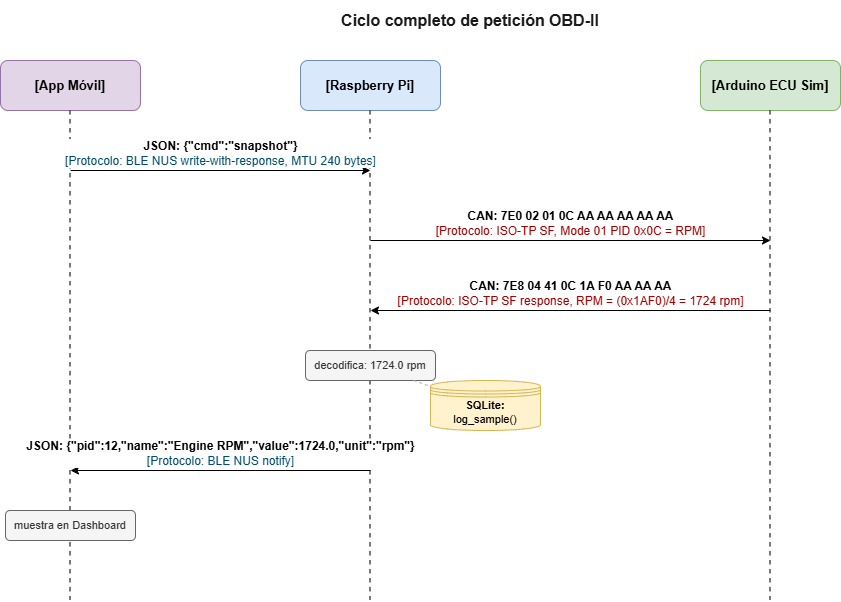
\includegraphics[width=0.9\textwidth]{Ilustraciones/obd2_cycle.png}
\caption{Ciclo completo de una petición OBD-II desde la aplicación móvil hasta la ECU. El comando JSON se transmite por BLE hasta la Raspberry Pi, que lo traduce a una trama ISO-TP/CAN, recibe la respuesta de la ECU, la decodifica, la persiste en SQLite y devuelve el resultado a la app.}
\label{fig:obd2_cycle}
\end{figure}
